%%%%                 %%%%
%%%% ESTADO DEL ARTE %%%%
%%%%                 %%%%

\chapter{Estado del arte}
\label{chap:estado-arte}

\lettrine{E}{n} este capítulo se exponen algunas soluciones comerciales que aplican en el mismo campo que este TFG. Antes de comentar las aplicaciones se explica cuales son las características habituales que se pueden encontrar y los conceptos relacionados. Se analizan también algunas publicaciones que tratan el problema de encontrar la información sin considerar el uso de plantillas.

\section{Soluciones comerciales}

\subsection{Funcionalidades comunes}

Son varias las soluciones comerciales que ofrecen capturar y generar información estructurada a partir de documentos estructurados o semiestructurados. En general, todas ellas se basan en los mismos conceptos, variando, por supuesto, el número y calidad de características disponibles, la flexibilidad de las opciones en cada caso, modo de implantación, costes, etc.

Tanto si se quieren tratar uno o varios documentos la unidad de trabajo es el lote o batch. En un lote se pueden tratar ciertos tipos de documentos y cada uno de estos documentos tendrá unas zonas de interés: los lugares donde se encuentra la información relevante. Los documentos pueden tener un número de páginas variable.

\begin{itemize}
    \item El flujo de información comienza cuando se \textbf{selecciona el tipo de batch} y el \textbf{origen de los documentos}. Orígenes puede haber muchos, por ejemplo un escáner, correos electrónicos o directorios monitorizados para la aparición de ficheros. Una vez adquirida la información desde la fuente configurada, los documentos son separados y clasificados. La separación se utiliza cuando el batch está preparado con múltiples documentos en el mismo lote. El software debe ser capaz de seleccionar qué páginas individuales pertenecen a cada documento. Las soluciones habituales emplean separadores físicos, páginas en blanco o códigos de barras, entre los de documentos. Como alternativa, pueden aprovecharse características particulares de los documentos, que el software debe ser capaz de detectar. Por ejemplo, es posible que en un tipo de documento, aparezca siempre un logotipo en la primera página y un determinado texto en la última. La clasificación relaciona un documento concreto con un tipo de documento tratable por el tipo de batch. Es el paso necesario para saber qué áreas geográficas deben ser extraídas.
    
    \item La \textbf{extracción de los datos} se lleva a cabo aplicando reglas sobre las zonas de los documentos. Cuando se configura un tipo de documento se indican tipos de regiones que lo componen. Los tipos más habituales son celdas o rectángulos individuales, pares clave-valor, tablas, códigos de barras de una o dos dimensiones, o logotipos. El usuario procede cargando un documento que sirva de modelo y se le presentan las páginas individuales en un visor donde puede definir los tipos de regiones seleccionando áreas con el ratón.
    
    \item Las dos últimas fases son la \textbf{validación de los resultados} y la \textbf{importación a terceros sistemas}. La validación tiene como objetivo detectar errores en los datos extraídos y notificar a los usuarios del sistema para el análisis y corrección de estos errores. Para la detección se emplean un conjunto de técnicas. La más sencilla consiste en detectar campos obligatorios que estén vacíos. Otra idea consiste en comprobar si se han aplicado correctamente los tipo de datos configurado a una celda o un par clave-valor. El campo se marcará para su revisión en caso de fallo. Esto se puede utilizar para las fechas o los importes, por ejemplo. Un caso más elaborado consiste en corregir o complementar la validación a partir de datos en bases de datos externas. Se puede utilizar para validar los datos de contacto de un cliente, razón social, dirección, teléfono; a partir de información parcial.
    
    La importación a terceros sistemas consiste en la publicación de los resultados en las bases de datos, sistemas ERP o cualquier otro software donde los datos puedan ser explotados. El caso más sencillo generará ficheros estructurados a un directorio particular. Estas salidas pueden ser en formato \emph{\acrlong{csv}} o \emph{\acrlong{xml}}/\emph{\acrlong{json}} para los documentos más complejos o imágenes.
\end{itemize}

Algunas de estas aplicaciones permiten definir roles para los usuarios. En un entorno empresariales es habitual establecer una separación de tareas que facilite la organización y simplifique la formación del personal. Algunos roles habituales son el de administrador, el rol para definir tipos de batch y tipos de documentos, el rol para crear, editar y eliminar trabajos batch y el rol de validación. Además, alguna de las soluciones puede implantarse con una arquitectura cliente-servidor donde puestos remotos generarán los nuevos procesos por lotes. Estos puestos remotos pueden ser las oficinas donde se trata con cliente o proveedores. Un nuevo lote creado se enviará para ser tratados por un conjunto de servidores en la central de la empresa y validados por personal especializado en esa tarea.

\subsection{Capture de Kofax y FlexiCapture}

Las dos soluciones con mayor número de características son FlexiCapture de Abbyy \cite{solucionesComerciales_abbyy_flexicapture4invoices} y Capture de Kofax \cite{solucionesComerciales_kofax_capture}. Se muestran en la Imagen \ref{fig:kofax-capture-y-abbyy-flexicapture}. Las dos tienen una larga lista de características entre las mencionadas anteriormente, están posicionadas para cubrir un amplio espectro de necesidades ya que se pueden instalar individualmente en un equipo de trabajo como pero pueden crecer para con una arquitectura cliente-servidor modular capaz de absorber grandes volúmenes de trabajos. Ambas soportan roles para los usuario. Estas empresas tienen catálogos de productos que complementan y/o amplían las funcionalidades básicas.

\begin{figure}
    \centering
    \begin{subfigure}[b]{0.9\textwidth}
        \centering
        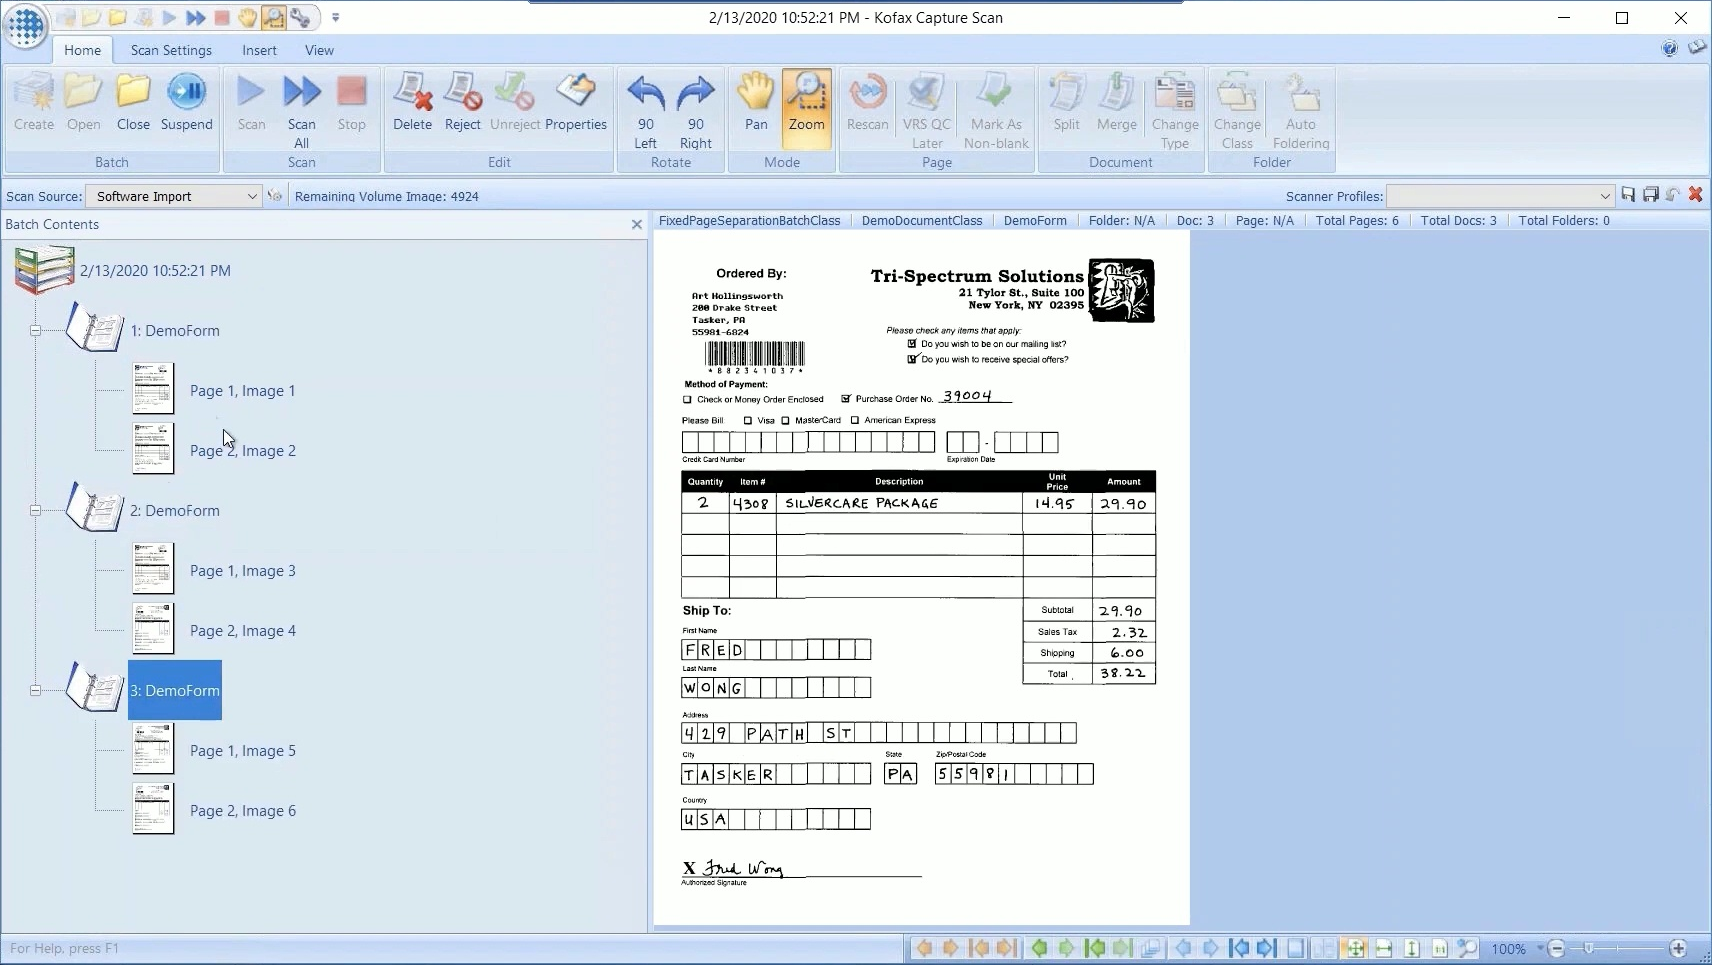
\includegraphics[width=\textwidth]{imaxes/b-estado-arte/kofax-capture}
        \label{fig:hough-punto-imagen}
    \end{subfigure}
    \begin{subfigure}[b]{0.9\textwidth}
        \centering
        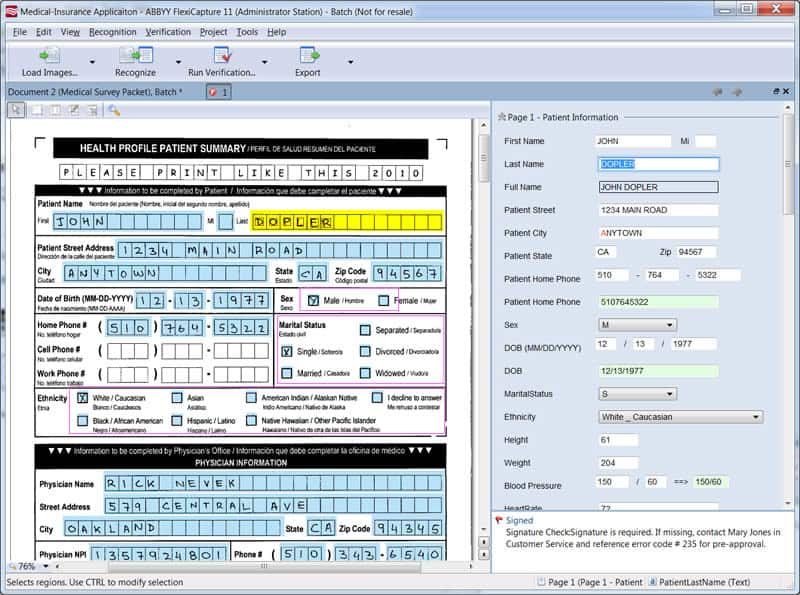
\includegraphics[width=\textwidth]{imaxes/b-estado-arte/abbyy-flexicapture}
        \label{fig:hough-intersection}
    \end{subfigure}
    \caption{Kofax Capture (arriba) y ABBYY FlexiCapture (abajo)}
    \label{fig:kofax-capture-y-abbyy-flexicapture}
\end{figure}

\subsection{Grooper}

Grooper \cite{solucionesComerciales_bisok_grooper} (ver Imagen \ref{fig:grooper-bisok}) está hecho por Bisok y a priori parece seguir próxima en características a las dos anteriores. No obstante durante la búsqueda de información ha llamado la atención la mala organización de la información en la web oficial donde no existe una página o documento lineal que explique las características de la aplicación. Una característica destacable es el uso de técnicas de Procesamiento de lenguajes naturales para encontrar párrafos y frases en un documento o ser capaz de distinguir las clausulas en un contrato. También permite seleccionar el engine de \emph{\acrlong{ocr}} utilizado entre un abanico de opciones.

\begin{figure}[hp!]
    \centering
    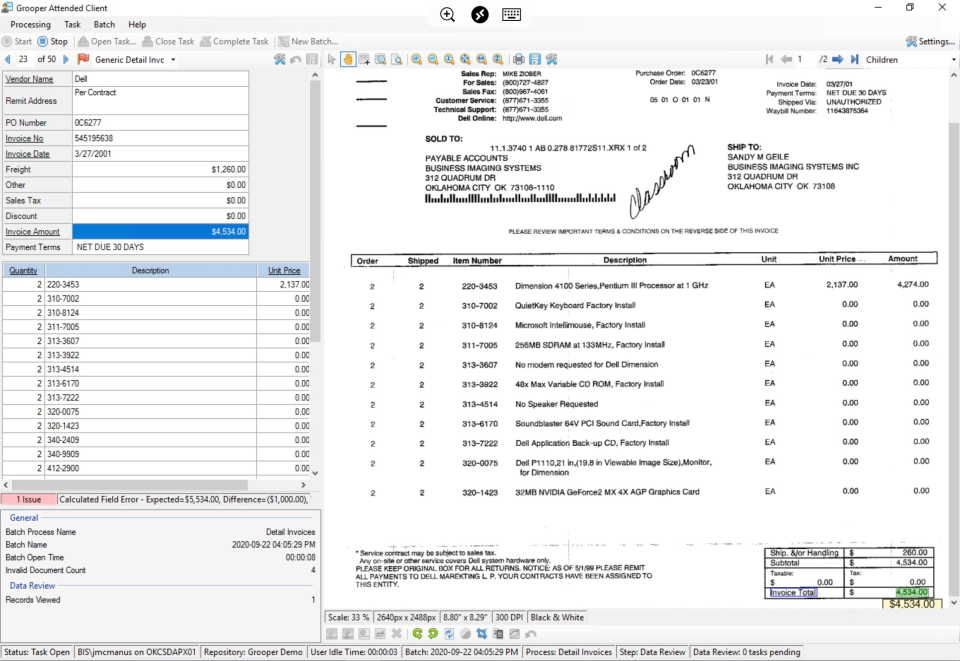
\includegraphics[width=0.9\textwidth]{imaxes/b-estado-arte/bisok-grooper}
    \caption{Grooper, la solución de Bisok}
    \label{fig:grooper-bisok}
\end{figure}

\subsection{Capture de ChronoScan}

Capture de ChronoScan \cite{solucionesComerciales_chronoScanCapture_chronoScanDocumentCapture} (ver Imagen \ref{fig:chronoscan-capture}) es una aplicación individual más limitada en funcionalidades que las anteriores. Soporta el flujo normal de lotes con documento pero no dispone de arquitectura cliente servidor por lo cual su uso puede ser más interesante para pequeñas empresas o usuarios individuales. En este sentido la licencia permite su uso sin restricciones siempre que no sea en un contexto profesional.

\begin{figure}[hp!]
    \centering
    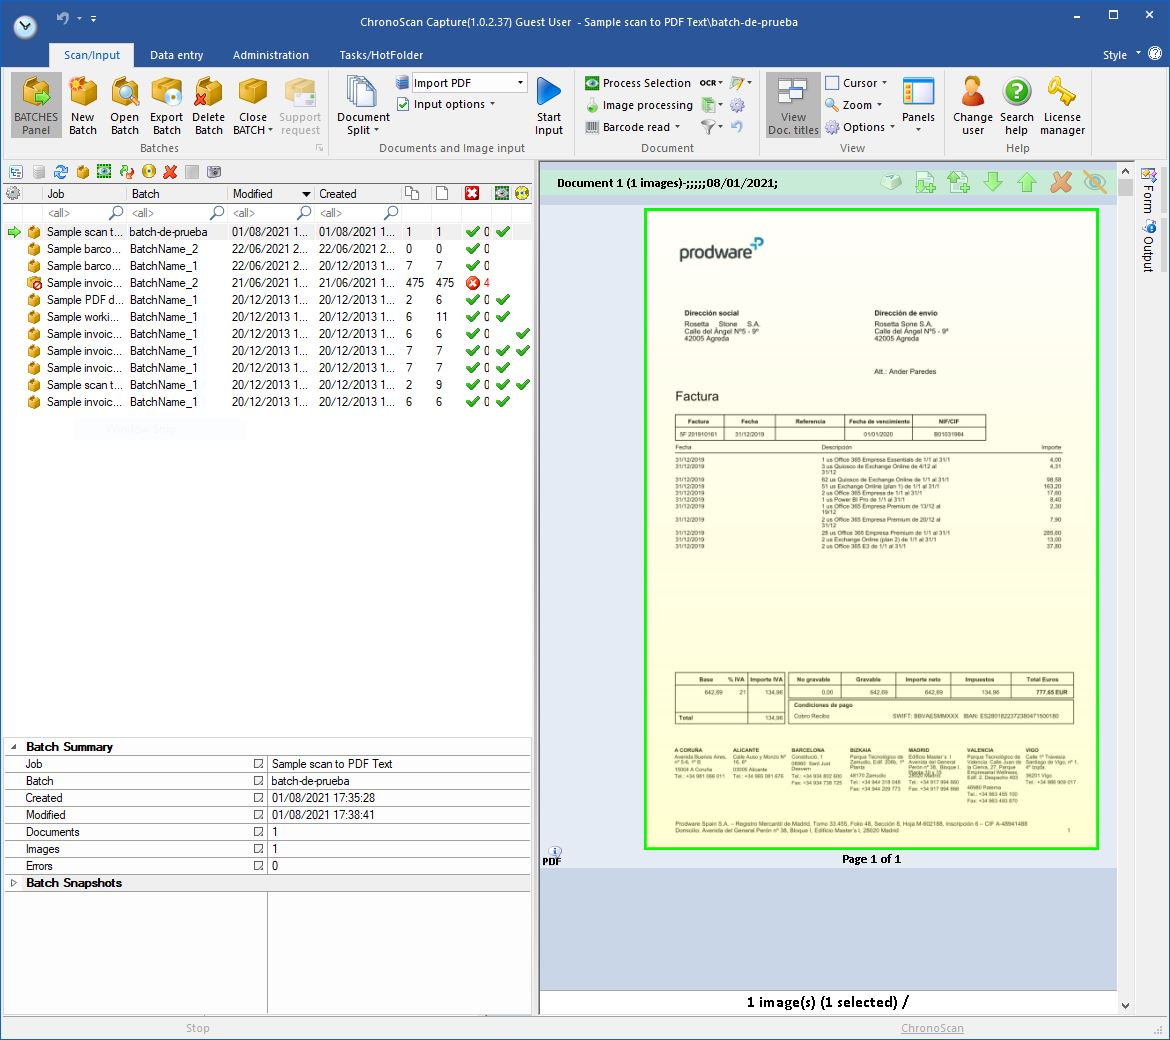
\includegraphics[width=0.8\textwidth]{imaxes/b-estado-arte/chronoscan-capture}
    \caption{ChronoscanCapture con uno de los documentos usando en el proyecto}
    \label{fig:chronoscan-capture}
\end{figure}

\subsection{DocAcquire}

DocAcquire \cite{solucionesComerciales_docAcquire_docAcquire} es una solución \emph{\acrlong{saas}} y no dispone de versión de escritorio. Se puede probar de forma gratuita acudiendo a la web oficial. Es la aplicación más simple de todas y, al menos en la versión de prueba, parece que las acciones están bastante limitadas. No se pueden eliminar tipos de documentos una vez creados. Utiliza en engine Tesseract para \acrshort{ocr}.

\subsection{Textract y Document AI}

Dos servicios diferentes a los productos anteriores pero aplicables al problema son, Textract de Amazon \cite{solucionesComerciales_amazon_textract} y Document AI de Google \cite{solucionesComerciales_google_documentAI}. Ninguno de los dos suporta el flujo de información explicado ni están pensados para ser solución para el usuario final. Lo que ofrecen es un \emph{\acrlong{api}} capaz de recibir documentos y generar información estructurada como salida. El caso de Textract es totalmente opaco y por tanto no configurable. La salida consiste en ficheros JSON donde puede haber varios tipos de objetos: páginas, líneas y palabras, información de formularios (pares clave-valor), tablas, y elementos seleccionables como casillas. Además es capaz de identificar notas manuscritas. El servicio de Google permite definir \emph{processors}, que son plantillas específicas para modelos de documentos concretos. Actualmente parece que el servicio es muy reciente y está mayormente en beta. Cualquiera de ellos podría utilizarse para construir una solución más completa. Como otros servicios en la nube, el coste depende de la carga de trabajo procesada.

Después de revisar todas estas alternativas uno de los elementos comunes es el procesado por lotes. En general se deja en manos de los usuarios definir cómo son los modelos de los documentos por medio de un editor que selecciona regiones fijas y les asigna una topología. Estas dos características apuntan a que el sistema.

\begin{figure}
    \centering
    \begin{subfigure}[b]{0.9\textwidth}
        \centering
        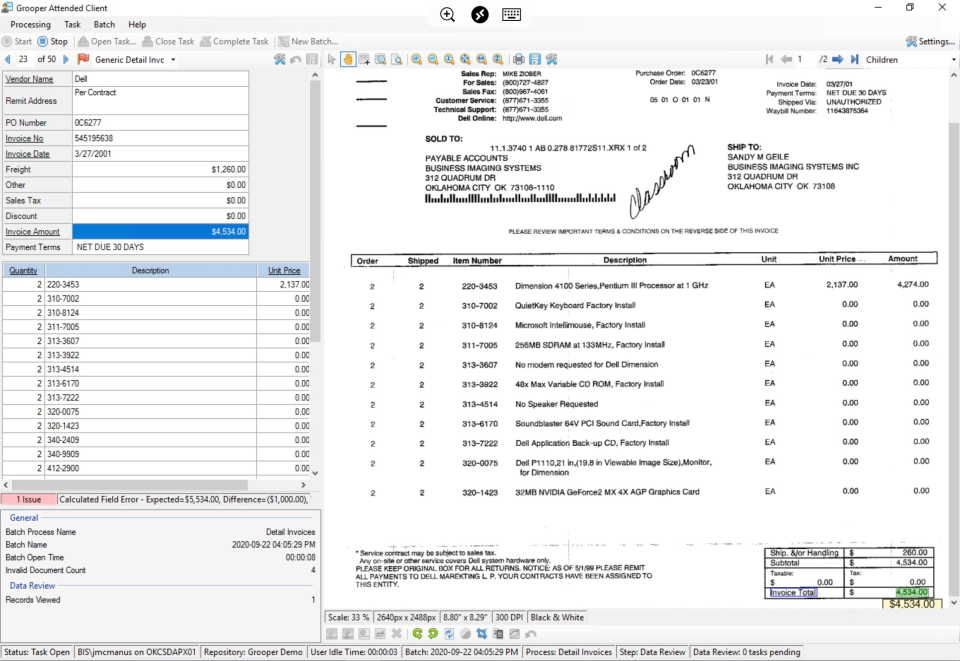
\includegraphics[width=\textwidth]{imaxes/b-estado-arte/bisok-grooper}
        \caption{Grooper, la solución de Bisok.}
        \label{fig:grooper-bisok}
    \end{subfigure}
    \begin{subfigure}[b]{0.8\textwidth}
        \centering
        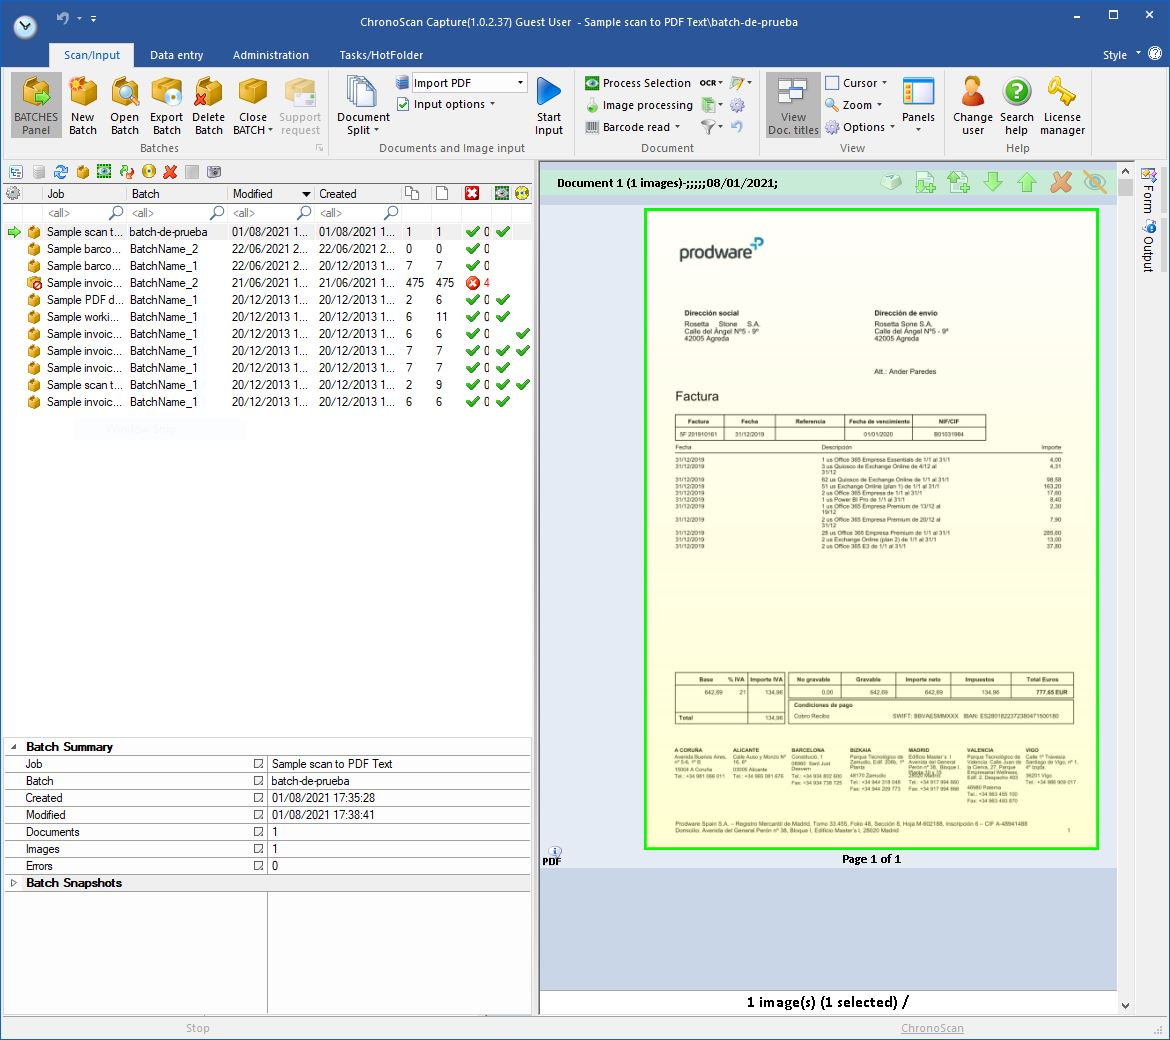
\includegraphics[width=\textwidth]{imaxes/b-estado-arte/chronoscan-capture}
        \caption{ChronoscanCapture con uno de los documentos usando en el proyecto.}
        \label{fig:chronoscan-capture}
    \end{subfigure}
%    \caption{Kofax Capture (arriba) y ABBYY FlexiCapture (abajo)}
%    \label{fig:grooper-y-chronoscan-capture}
\end{figure}
